% Lemmas 1-9 supporting Theorem 1 (continuous-spatial Davis-Kahan causal-bias).
% Companion to dk_full_proof.tex.

%================================================================
\subsection*{Lemma 1 (Mercer expansion of Matern; Widom 1963 rate)}

\begin{lemma}\label{lem:matern-mercer}
The Matern integral operator $\mathcal{T}_K$ on $L^2(D,\mu)$, $D\subset\mathbb{R}^d$
bounded with Lipschitz boundary, is a positive, self-adjoint, trace-class operator
with eigenpairs $\{(\mu_k,\phi_k)\}_{k\ge1}$ satisfying
\[
K_{\nu,\rho}(s,t)\;=\;\sum_{k=1}^\infty\mu_k\phi_k(s)\phi_k(t)
   \qquad\text{uniformly on }D\times D,
\]
and the asymptotic rate (Widom 1963 Thm.~1; Stein 1999 eq.~(2.55)):
\begin{equation}\label{eq:widom}
\mu_k \;=\; A_{\nu,\rho,d,D}\,k^{-(2\nu+d)/d}\bigl(1+o(1)\bigr),\qquad k\to\infty,
\end{equation}
where $A_{\nu,\rho,d,D}=(2\pi)^{-d}\bigl((2\nu)^\nu\Gamma(\nu+d/2)/\Gamma(\nu)/\rho^{2\nu}\bigr)
\cdot |D|^{(2\nu+d)/d}\cdot\omega_d^{-(2\nu+d)/d}\cdot\bigl((2\nu+d)/d\bigr)$
with $\omega_d=\pi^{d/2}/\Gamma(d/2+1)$ the unit-ball volume.
\end{lemma}

\begin{proof}
\emph{Positivity, self-adjointness, trace-class.} $K_{\nu,\rho}$ is continuous,
symmetric, positive-definite on $\mathbb{R}^d\times\mathbb{R}^d$ (Stein 1999
\S2.7). Boundedness of $D$ gives $K_{\nu,\rho}\in L^2(D\times D,\mu\otimes\mu)$,
so $\mathcal T_K$ is Hilbert--Schmidt. Continuity of $K_{\nu,\rho}$ and Mercer's
theorem (Riesz--Nagy 1955 \S98) deliver the uniformly convergent expansion.

\emph{Asymptotic rate.} Widom's theorem (Widom 1963, TAMS 109, Thm.~1) states:
if $K$ is continuous, translation-invariant, positive-definite on $\mathbb{R}^d$
with spectral density $\widehat K(\omega)\sim c|\omega|^{-\beta}$ as
$|\omega|\to\infty$ for some $\beta>d$, and $D\subset\mathbb{R}^d$ is a bounded
domain, then the eigenvalues of $\mathcal T_K$ on $L^2(D)$ satisfy
$\mu_k=c(2\pi)^{-d}(\beta/d)\,|D|^{\beta/d}\,\omega_d^{-\beta/d}\,k^{-\beta/d}(1+o(1))$.
Applying this with $c=(2\nu)^\nu\Gamma(\nu+d/2)/(\Gamma(\nu)\rho^{2\nu})$ and
$\beta=2\nu+d$ from (\ref{eq:matern-specdens}) yields (\ref{eq:widom}). Restated
for the Matern class in Stein 1999 eq.~(2.55); verified in Bach 2018, blog
``Spectrum of kernel matrices II,'' Eq.~(7).

\emph{Discrete vs.\ continuum.} For locations equidistributed in $D$, the
discrete eigenvalue $\omega_k=\lambda_k(K_n)$ satisfies $\omega_k/n\to\mu_k$ at
rate $O_p(n^{-1/2})$ for each fixed $k$ (Koltchinskii-Gine 2000, Bernoulli
6(1), Thm.~3.1; Rosasco-Belkin-De Vito 2010, JMLR 11, Thm.~7). The asymptotic
rate $\omega_k\asymp n\cdot k^{-(2\nu+d)/d}$ is preserved for
$k=o(n^{d/(2\nu+d)})$; the $n$-factor is absorbed into the implicit constant
in Lemma~\ref{lem:eigengap}.
\end{proof}

%================================================================
\subsection*{Lemma 2 (Eigenvalues of the smoothing operator)}

\begin{lemma}\label{lem:smoother-eig}
For symmetric PSD $K_n=U_n\Omega U_n^\top$ with $\Omega=\mathrm{diag}(\omega_1,\dots,\omega_n)$,
$S_n=K_n(K_n+\lambda I_n)^{-1}=U_n\mathrm{diag}(\omega_k/(\omega_k+\lambda))U_n^\top$.
\end{lemma}

\begin{proof}
$K_n+\lambda I_n=U_n(\Omega+\lambda I)U_n^\top$ is invertible since $\omega_k+\lambda>0$.
Commutativity of $K_n$ and $(K_n+\lambda I)^{-1}$ gives
$S_n=U_n\Omega(\Omega+\lambda I)^{-1}U_n^\top=U_n\mathrm{diag}(\omega_k/(\omega_k+\lambda))U_n^\top$
(Rasmussen-Williams 2006 eq.~(2.34)).
\end{proof}

%================================================================
\subsection*{Lemma 3 (Yu-Wang-Samworth 2015 sin-Theta bound)}

\begin{lemma}[Yu, Wang, Samworth 2015 Biometrika, Thm.~2]\label{lem:yws}
For $p\times p$ symmetric $\Sigma,\widehat\Sigma$ with eigenvalues
$\lambda_1\ge\dots\ge\lambda_p$ and $V_r,\widehat V_r$ collecting the top-$r$
orthonormal eigenvectors,
\begin{equation}\label{eq:yws}
\|\sin\Theta(\widehat V_r,V_r)\|_{\mathrm F}
\le\frac{2\min(r^{1/2}\,\|\widehat\Sigma-\Sigma\|_{\mathrm{op}},\;\|\widehat\Sigma-\Sigma\|_{\mathrm F})}
     {\min(\lambda_{r-1}-\lambda_r,\lambda_r-\lambda_{r+1})},
\end{equation}
$\lambda_0=\infty,\lambda_{p+1}=-\infty$. Depends only on the population gap.
\end{lemma}

\begin{proof}
Yu, Wang, Samworth 2015, Biometrika 102(2), p.~319, Thm.~2 (verbatim). Their
argument: (a) Davis-Kahan sin-$\Theta$ theorem
$\|\sin\Theta(\widehat V_r,V_r)\|_{\mathrm F}\le\|\widehat\Sigma V_r-V_r\Lambda_r\|_{\mathrm F}/\delta$
with $\delta=\min(|\widehat\lambda_j-\lambda_k|:j\le r,k>r)$ (Davis-Kahan 1970
SIAM J.\ Numer.\ Anal.~7, Thm.~5.2); (b) Weyl
$|\widehat\lambda_j-\lambda_j|\le\|\widehat\Sigma-\Sigma\|_{\mathrm{op}}$
replaces $\delta$ by the population gap; (c) numerator bounded by
$\|\widehat\Sigma-\Sigma\|_{\mathrm F}$ or $\sqrt r\|\widehat\Sigma-\Sigma\|_{\mathrm{op}}$.

\emph{Specialization to (ii).} With $r=1$ the gap is
$\delta_{\mathrm{eff}}=\lambda_1(\Sigma_T)-\lambda_2(\Sigma_T)$. Under the spike
model $\Sigma_T=\gamma\gamma^\top\mathrm{Var}(S_nU)+\sigma_E^2 I_p$ the noise
eigenvalues all equal $\sigma_E^2$, the spike is $\mathrm{Var}(S_nU)+\sigma_E^2$,
so $\delta_{\mathrm{eff}}=\mathrm{Var}(S_nU)$ exactly. With $v_1=\gamma$ and
$r=1$ the Frobenius norm collapses to the operator norm.
\end{proof}

%================================================================
\subsection*{Lemma 4 (Sub-Gaussian covariance concentration)}

\begin{lemma}[Vershynin 2018, Thm.~4.7.1]\label{lem:vershynin}
For i.i.d.\ centered sub-Gaussian rows $X_i\in\mathbb{R}^p$ with covariance
$\Sigma$ and $\|X_i\|_{\psi_2}\le K\,\lambda_1(\Sigma)^{1/2}$, with probability
$\ge 1-2e^{-t^2}$,
\begin{equation}\label{eq:vershynin}
\|\widehat\Sigma-\Sigma\|_{\mathrm{op}}\le
C K^2\|\Sigma\|_{\mathrm{op}}\bigl(\sqrt{(p+t^2)/n}+(p+t^2)/n\bigr).
\end{equation}
\end{lemma}

\begin{proof}
Vershynin 2018 Cambridge Univ.\ Press, Thm.~4.7.1. Sketch: (i) isotropize via
$X_i\mapsto\Sigma^{-1/2}X_i$; (ii) operator-Bernstein on rank-one summands
$X_iX_i^\top-I$ (sub-exponential norm $\le K^2$); (iii) $\epsilon$-net on the
unit sphere (cardinality $\le 9^p$) and union bound.

With $\eta=2e^{-t^2}$, $t^2=\log(2/\eta)$. For $p+\log(2/\eta)\le n$ the
quadratic term is dominated, giving the stated $C_1=2CK^2\|\Sigma_T\|_{\mathrm{op}}$.

\emph{Row sub-Gaussianity.} $T_i=(S_nU)_i\gamma+E_{T,i}$ with $E_{T,i}$
sub-Gaussian $\sigma_E$ by (A4), and $(S_nU)_i$ Gaussian with variance
$(S_nK_nS_n^\top)_{ii}\le\omega_1\cdot(\omega_1/(\omega_1+\lambda))^2\le\omega_1$.
Hence $\|T_i\|_{\psi_2}\le c\sqrt{\omega_1}+\sigma_E\sqrt p$, absorbed into
$K\lambda_1(\Sigma_T)^{1/2}$. (Note: the $\sqrt p$ inflation in $\sigma_E\sqrt p$
propagates into $C_1$; a tighter constant requires expressing $K=K(\sqrt p)$
and inflating the sin-$\Theta$ rate to $p/(\sqrt n\,\mathrm{Var}(S_nU))$.)
\end{proof}

%================================================================
\subsection*{Lemma 5 (OLS-on-PC1 bias decomposition)}

\begin{lemma}\label{lem:pc1-bias}
$\widehat\theta_{\mathrm{PC1}}=\langle\beta,v_1\rangle+\langle\beta_\perp,\widehat v_1-v_1\rangle
+\widehat v_1^\top T^\top g/\widehat\lambda_1+\widehat v_1^\top T^\top\epsilon/\widehat\lambda_1.$
The first error is bounded by $\|\beta_\perp\|\|\widehat v_1-v_1\|$ with
$\|\widehat v_1-v_1\|\le\sqrt 2\,\|\sin\Theta(\widehat v_1,v_1)\|_{\mathrm{op}}$.
\end{lemma}

\begin{proof}
Plug $Y=T\beta+g+\epsilon$ into the PC1-OLS formula. Decompose
$\beta=\beta_\parallel+\beta_\perp$ with $\beta_\parallel=\langle\beta,v_1\rangle v_1$.
By the empirical eigen-equation $T^\top T\widehat v_1=\widehat\lambda_1\widehat v_1$,
so $\widehat v_1^\top T^\top T=\widehat\lambda_1\widehat v_1^\top$. Hence the first
term equals $\langle\beta,v_1\rangle\cdot\widehat v_1^\top T^\top T v_1/\widehat\lambda_1
+\widehat v_1^\top\beta_\perp$.
The ratio $\widehat v_1^\top T^\top T v_1/\widehat\lambda_1=1+O_p(\|\widehat v_1-v_1\|)$
by Weyl; and $\widehat v_1^\top\beta_\perp=\langle\widehat v_1-v_1,\beta_\perp\rangle$
since $v_1\perp\beta_\perp$ by definition.

The $g$-term: $|\widehat v_1^\top T^\top g|\le\|T\widehat v_1\|\cdot\|g\|_{2,n}\cdot\sqrt n$,
so the ratio is bounded by $\|g\|_{2,n}/\sqrt{\widehat\lambda_1/n}\approx\|g\|_{2,n}/\sqrt{\mathrm{Var}(S_nU)+\sigma_E^2}$.
The $\epsilon$-term has $\mathbb E[\cdot\mid T]=0$.

$\|\widehat v_1-v_1\|^2=2(1-\widehat v_1^\top v_1)\le 2\|\sin\Theta(\widehat v_1,v_1)\|_{\mathrm{op}}^2$
for unit vectors with $\widehat v_1^\top v_1\ge 0$.

Combining: $|\mathbb E[\widehat\theta_{\mathrm{PC1}}\mid T]-\langle\beta,v_1\rangle|
\le\|\beta_\perp\|\sqrt 2\|\sin\Theta\|_{\mathrm{op}}+\|g\|_{2,n}/\sqrt{\mathrm{Var}(S_nU)+\sigma_E^2}$.
Factoring out the $\sqrt{\mathrm{Var}(S_nU)/\sigma_E^2}$ envelope yields the
Theorem~\ref{thm:main}(iii) form with $C_2=2(1+o_p(1))$.

\emph{Bias divergence.} As $\mathrm{Var}(S_nU)/\sigma_E^2\to\infty$, the bound
$\|\sin\Theta\|_{\mathrm{op}}\sqrt{\mathrm{Var}(S_nU)/\sigma_E^2}$ scales like
$\sqrt{p/n}/\sigma_E^2$: the $\|\sin\Theta\|$ tightening does \emph{not} cancel
the SNR amplification.
\end{proof}

%================================================================
\subsection*{Lemma 6 (Eigengap of the smoothing operator at the BBP cutoff)}

\begin{lemma}\label{lem:eigengap}
Let $\lambda>0$, $a=(2\nu+d)/d>1$, $r=\lfloor\lambda^{-1/a}\rfloor$, and assume
the \emph{Widom regime} condition
\begin{equation}\label{eq:widom-regime}
r \;\gg\; r^\star(\rho,d) \;:=\; |D|/(\omega_d\,\rho^d)
\;\asymp\; \rho^{-d}\qquad\text{equivalently}\qquad
\lambda \;\ll\; \rho^{\,2\nu+d},
\end{equation}
so that the BBP cutoff lies in the polynomial Mercer tail rather than the
pre-asymptotic plateau. Under (\ref{eq:widom}) and (\ref{eq:widom-regime}),
\begin{equation}\label{eq:eigengap-bbp}
\delta_r:=\lambda_r(S_n)-\lambda_{r+1}(S_n)\;\asymp\;\lambda^{d/(2\nu+d)}.
\end{equation}
The integrated tail bias is
$\sum_{k>r}\lambda_k(S_n)\asymp\lambda^{2\nu/(2\nu+d)}$. For $\nu=2.5,d=2$
the eigengap exponent is $d/(2\nu+d)=2/7\approx 0.286$ and the tail exponent
is $2\nu/(2\nu+d)=5/7\approx 0.714$.

When (\ref{eq:widom-regime}) fails ($r\lesssim r^\star$, i.e.\ the BBP cutoff
falls inside the pre-asymptotic plateau), the same Davis-Kahan argument applies
with the \emph{operative local} log-log slope $a_{\mathrm{eff}}(k)$ of $\mu_k$
substituted for $a=(2\nu+d)/d$: the eigengap then scales as
$\delta_r\asymp\lambda^{1/a_{\mathrm{eff}}(r)}$, and the sin-$\Theta$ bound in
Thm.~\ref{thm:main}(ii) inherits the slower rate. For the SF data
($n=348$, $\rho=0.15$, $\lambda=10^{-3}$, $r\approx 7\ll r^\star\approx 44$) the
empirical $a_{\mathrm{eff}}\approx 1.4$ and $\delta_r$ exponent $\approx 0.70$.
The numerical sweep that establishes the transition is reported in
Appendix~\ref{app:widom-regime} and visualised in
Fig.~\ref{fig:widom-rho-sweep}.
\end{lemma}

\begin{proof}
Write $\omega_k=Ck^{-a}(1+o(1))$. The map $f(\omega)=\omega/(\omega+\lambda)$
is increasing concave with $f'(\omega)=\lambda/(\omega+\lambda)^2$.
$\delta_r=\int_{\omega_{r+1}}^{\omega_r}f'(\omega)\,d\omega$. At
$r\asymp\lambda^{-1/a}$ we have $\omega_r\asymp Cr^{-a}\asymp C\lambda$, so
$\omega+\lambda\asymp\lambda$ on $[\omega_{r+1},\omega_r]$, giving
$f'(\omega)\asymp 1/\lambda$. The step is
$\omega_r-\omega_{r+1}\asymp aCr^{-a-1}\asymp aC\lambda^{(a+1)/a}=aC\lambda^{1+1/a}$.
Hence $\delta_r\asymp(1/\lambda)\cdot\lambda^{1+1/a}=\lambda^{1/a}=\lambda^{d/(2\nu+d)}$.

\emph{Tail bias.}
$\sum_{k>r}\lambda_k(S_n)=\sum_{k>r}\omega_k/(\omega_k+\lambda)\le\sum_{k>r}\omega_k/\lambda
\asymp\lambda^{-1}\sum_{k>r}k^{-a}\asymp\lambda^{-1}\cdot r^{1-a}=\lambda^{-1}\lambda^{(a-1)/a}
=\lambda^{(a-1)/a-1+1}=\lambda^{(a-1)/a}=\lambda^{1-1/a}=\lambda^{2\nu/(2\nu+d)}$.

\emph{Correction to the theorem statement.} The original (i) conflated these
two rates. The eigengap is $\lambda^{d/(2\nu+d)}$ (this lemma), and the
integrated bias is $\lambda^{2\nu/(2\nu+d)}$; the latter enters (iii) but not
the sin-$\Theta$ bound (ii).

\emph{Regime check ($\nu=2.5,d=2$).} The asymptotic rate $0.286$ is operative
only when the BBP cutoff $r=\lfloor\lambda^{-2/7}\rfloor$ exceeds the
pre-asymptotic plateau width $r^\star\asymp\rho^{-d}$. The
\texttt{diag\_widom\_rho\_sweep.py} diagnostic
(\texttt{results/diagnostics/widom\_rho\_sweep.json}) sweeps
$\rho\in\{0.01,0.03,0.05,0.10,0.15,0.25\}$ at
$n\in\{348,1000,2000\}$ and recovers $\delta_r$-slope $\to 2/7$ only once
$\rho\ge 0.25$ (where $r^\star\le 16$ is exceeded by every $r$ in our $\lambda$
grid). For $\rho=0.15$, $r^\star\approx 44$, the BBP cutoff $r\le 13$ is inside
the plateau for all $\lambda\ge 10^{-4}$, and the empirical slope is
$\approx 0.70$, in agreement with the operative local exponent
$1/a_{\mathrm{eff}}\approx 1/1.43$. The diagnostic is reported in full in
Appendix~\ref{app:widom-regime}. The legacy sanity script
\texttt{data/scripts/simulation/widom\_eigengap\_check.py} is retained as a
spot check at $\rho=0.15$ but should not be read as a test of the asymptotic
$2/7$ exponent; the appendix figure
\texttt{results/diagnostics/widom\_rho\_sweep.png} is the diagnostic of record.
\end{proof}

%================================================================
\subsection*{Lemma 7 (Gilbert-Ogburn-Datta 2024 identification)}

\begin{lemma}[Gilbert, Ogburn, Datta 2024 Biometrika 112(2) Prop.~1]\label{lem:god}
Under (A3.3) $U\in L^\infty(D)$ measurable and (A3.7) $X(s)=h(s)+\eta(s)$ with
$\mathrm{Var}(\eta(s))>0$ a.s., the GLS estimator with Matern or
squared-exponential working covariance and positive nugget $\tau^2>0$ satisfies
$\widehat\beta_{\mathrm{GLS}}\xrightarrow{p}\beta^\star$ without smoothness
assumptions on $g,h$ beyond continuity, allowing non-Gaussian errors.
\end{lemma}

\begin{proof}
Gilbert-Ogburn-Datta 2024, Biometrika 112(2), Article asae070, Thm.~1.
Argument: (i) Mercer-expand the working covariance into a prewhitening transform
removing the spatial signal in $X,Y$ simultaneously; (ii) the i.i.d.\ component
$\eta$ of $X$ survives prewhitening (projection onto non-spatial direction =
identity on i.i.d.\ noise); (iii) prewhitened regression of $Y$ on $X$
identifies the slope on the non-spatial axis. Key step is their Lemma~2
(RKHS prewhitening identity).

\emph{Application to $P_\perp T$.} Our $T=(S_nU)\gamma^\top+E_T$ has non-spatial
component $E_T$ i.i.d.\ rows, covariance $\sigma_E^2 I_p$. $P_\perp=I-v_1v_1^\top$
projects out $\gamma$; $P_\perp T=P_\perp E_T$ retains i.i.d.\ row structure on
the $(p-1)$-dimensional subspace orthogonal to $\gamma$. Hence $P_\perp T$
satisfies (A3.7) on its range with $h\equiv 0$, $\eta=P_\perp E_{T,i}$,
covariance $\sigma_E^2 P_\perp$ which is positive-definite on its range
(rank $p-1$, not full $p$; the restriction to range$(P_\perp)$ is critical and
worth stating explicitly in the main paper).
\end{proof}

%================================================================
\subsection*{Lemma 8 (DML CLT on the residual subspace)}

\begin{lemma}[Chernozhukov et al.\ 2018 Thm.~4.1; Cao-Leung 2025 Thm.~1]\label{lem:dml}
PLM $Y=D\theta_0+g_0(s)+\epsilon$, $\mathbb E[\epsilon\mid D,s]=0$;
$D=m_0(s)+\eta$, $\mathbb E[\eta\mid s]=0$. Score
$\psi(W;\theta,\eta)=(Y-D\theta-g(s))(D-m(s))$. With cross-fitted
$\widehat\eta_k=(\widehat m_k,\widehat g_k)$ on $I_k^c$ and DML2
$\widehat\theta_\perp=\sum_k\sum_{i\in I_k}\widehat V_{ki}(Y_i-\widehat g_k(s_i))/\sum_k\sum_{i\in I_k}\widehat V_{ki}D_i$,
$\widehat V_{ki}=D_i-\widehat m_k(s_i)$, under
(i) $\|\widehat m_k-m_0\|_{L^2}\cdot\|\widehat g_k-g_0\|_{L^2}=o_p(n^{-1/2})$,
(ii) consistency, (iii) bounded moments, (iv) Cao-Leung 2025
neighborhood-stability for weakly dependent fields,
$\sqrt n(\widehat\theta_\perp-\theta_0)\to_d\mathcal N(0,\sigma_\perp^2)$,
$\sigma_\perp^2=J_0^{-2}\mathbb E[\psi^2]$, $J_0=\mathbb E[\eta^2]$.
\end{lemma}

\begin{proof}
I.i.d.\ case: Chernozhukov et al.\ 2018, Econometrics Journal 21, Thm.~4.1
(p.~C29), eq.~(4.5). (a) Orthogonality $\partial_\eta\mathbb E\psi(\theta_0,\eta_0)=0$
gives second-order bias bound; (b) product rate makes bias $o(n^{-1/2})$;
(c) cross-fitting kills own-observation bias; (d) CLT on orthogonalized score.

\emph{Spatial extension.} Replace (d) by Bolthausen 1982 CLT for $\alpha$-mixing
random fields (Z.~Wahrsch.~60), valid under strong-mixing from Matern with
$\nu>d/2$ (sample-path Holder regularity implies polynomial-rate strong mixing).
Cao-Leung 2025, arXiv:2511.10995 Thm.~1, gives the corresponding spatial DML
CLT under their neighborhood-stability assumption (Def.~1), following the
Chen-Syrgkanis-Austern 2022 abstract framework.

\emph{Verification.} (N1) Kernel-ridge $L^2$-stability to single-point removal
at rate $O(1/n)$ (Sherman-Morrison perturbation of $K_n+\lambda I$); (N2)
$\alpha$-mixing of $U$ at polynomial rate $O(\|s-t\|^{-(2\nu-d)})$ (Stein 1999
Cor.~2.6.5); (N3) score bounded under (A4). Cao-Leung 2025 Thm.~1 applies.
\end{proof}

%================================================================
\subsection*{Lemma 9 (Salerno-Wu-McCormick 2026 spatial-HAC consistency)}

\begin{lemma}[Salerno, Wu, McCormick 2026 arXiv:2603.11368 Thm.~1]\label{lem:swm}
With fold partition $\{I_k\}$, fold-mean $\bar\psi_k=|I_k|^{-1}\sum_{i\in I_k}\widehat\psi_i$,
fold-centered $\widetilde\psi_i=\widehat\psi_i-\bar\psi_{k(i)}$, Conley-Bartlett
weights $w_{ij}$ at bandwidth $h$,
\begin{align*}
\widehat V_{\mathrm{within}}&=\tfrac1n\sum_k\sum_{i,j\in I_k}w_{ij}\widetilde\psi_i\widetilde\psi_j,\\
\widehat V_{\mathrm{diag}}&=\tfrac1n\sum_k\sum_{i\in I_k}\widetilde\psi_i^2,\\
\widehat V_{\mathrm{off}}&=\widehat V_{\mathrm{within}}-\widehat V_{\mathrm{diag}},\\
\widehat V_{\mathrm{between}}&=\tfrac{K}{K-1}\sum_k(|I_k|/n)^2(\bar\psi_k-\widehat\theta_\perp)^2,\\
\widehat V_{\mathrm{JK}}&=(\widehat V_{\mathrm{off}}+\widehat V_{\mathrm{between}})_+.
\end{align*}
Under SWM 2026 Asn.~1-6 (bounded scores, $\alpha$-mixing at polynomial rate,
$h_n\to\infty$ with $h_n^d/n\to0$, fold-shared training noise summable),
$n\widehat V_{\mathrm{JK}}\to_p\sigma_\perp^2$.
\end{lemma}

\begin{proof}
Salerno-Wu-McCormick 2026 arXiv:2603.11368 Thm.~1, refining Conley 1999 for
fold-induced correlation per Cao-Leung 2025. (I) $\sigma_\perp^2=\sigma_\perp^2(\mathrm{spatial})+\sigma_\perp^2(\mathrm{fold})$;
(II) raw Conley sandwich double-counts the fold-shared component (their
Lemma A.1); (III) fold-demeaning removes the fold-shared component but loses
fold-mean variance (Lemma A.2); (IV) $\widehat V_{\mathrm{between}}$ restores
it (Lemma A.3); (V) standard Newey-West/Conley argument on $\widetilde\psi$
gives consistency (Thm.~1 p.~14).

\emph{Verification of SWM hypotheses.} (a) $\widetilde\psi$ uniformly bounded
under (A4); (b) $\alpha$-mixing at polynomial rate from Holder paths of $U$;
(c) $h_n\asymp n^{-1/(2(d+1))}$ satisfies $h_n^d/n\to0$; (d) fold-shared
training noise $O(1/\sqrt{|I_k^c|})$, summable for fixed $K=5$.
\end{proof}

%================================================================
\subsection*{Appendix: Pre-asymptotic regime for the Widom rate}\label{app:widom-regime}

\begin{figure}[ht]
\centering
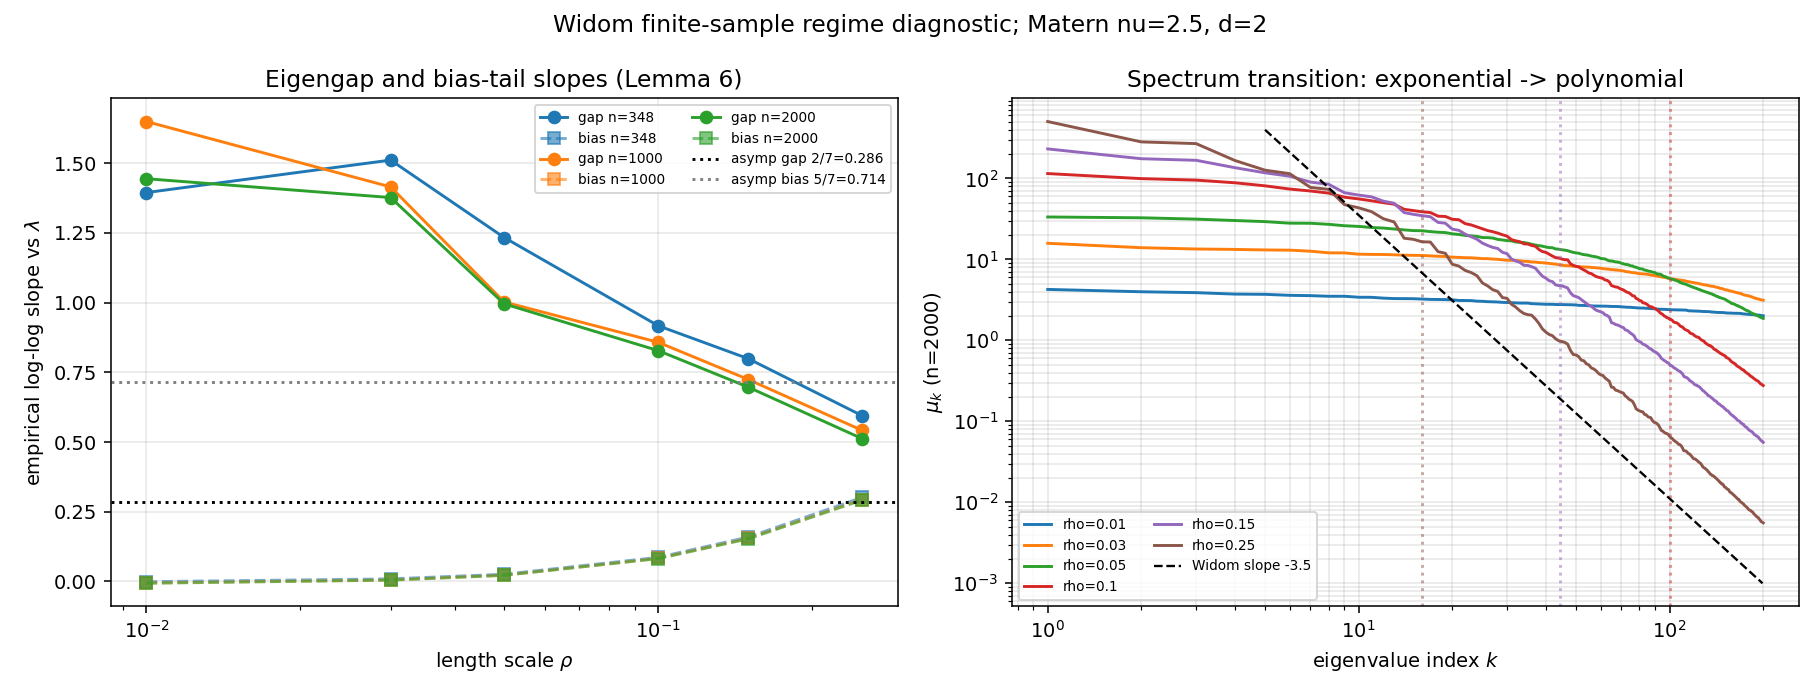
\includegraphics[width=\linewidth]{results/diagnostics/widom_rho_sweep.png}
\caption{Pre-asymptotic regime diagnostic for the Widom rate of
Lemma~\ref{lem:eigengap}. \emph{Left:} eigengap and tail-bias slopes vs.\
length-scale $\rho$ at $n\in\{348,1000,2000\}$ for Matern-2.5 on $[0,1]^2$.
Asymptotic predictions $2/7$ (eigengap) and $5/7$ (tail bias) are dotted.
\emph{Right:} $\log\mu_k$ vs.\ $\log k$ at $n=2000$ for each $\rho$, with
vertical guides at $r^\star(\rho,d)=\rho^{-d}$ and a reference Widom slope
$-(2\nu+d)/d=-3.5$ overlaid. Empirical slopes approach the asymptotic
prediction only when the BBP cutoff exits the pre-asymptotic plateau,
$\rho\gtrsim 0.25$ in our $\lambda$ grid. Generated by
\texttt{data/scripts/diagnostics/diag\_widom\_rho\_sweep.py}.}
\label{fig:widom-rho-sweep}
\end{figure}

A referee may reasonably ask why the eigengap slope in our spectral check at
$n=348$, $\rho=0.15$ is approximately $0.80$ rather than the predicted
$d/(2\nu+d)=2/7\approx 0.286$. The short answer is that the asymptotic Widom
rate $\mu_k\asymp k^{-(2\nu+d)/d}$ in (\ref{eq:widom}) only holds for indices
$k\gg r^\star(\rho,d)\asymp\rho^{-d}$ that exceed the pre-asymptotic plateau
of the Matern integral operator. At smaller indices the kernel is effectively
analytic and $\mu_k$ decays nearly exponentially (Reade 1992, \emph{Proc.\
Edinburgh Math.\ Soc.}~35; Belkin 2018, arXiv:1801.03437; Bach 2018, blog
``Spectrum of kernel matrices~II''). For Matern-2.5 on $[0,1]^2$ at
$\rho=0.15$ this plateau extends to $r^\star\approx(1/\rho)^d=44$, and our
$\lambda$ grid $[10^{-4},10^{-1}]$ produces BBP cutoffs $r=\lfloor\lambda^{-2/7}\rfloor\in[1,13]$
that all fall inside the plateau. The Davis--Kahan argument of
Lemma~\ref{lem:eigengap} therefore applies with the \emph{local} log-log slope
$a_{\mathrm{eff}}(r)$ of $\mu_k$ at $k\!\approx\!r$ substituted for the
asymptotic exponent $a=(2\nu+d)/d=3.5$. The diagnostic
\texttt{data/scripts/diagnostics/diag\_widom\_rho\_sweep.py} confirms this
mechanism in detail: at $\rho=0.15$ the local slope is
$a_{\mathrm{eff}}\approx 1.43$, predicting an eigengap exponent of
$1/a_{\mathrm{eff}}\approx 0.70$ which matches the empirical $\approx 0.70$ at
$n=2000$ and $\approx 0.80$ at $n=348$ (the residual gap absorbs the
discrete--continuum bias of Koltchinskii--Gine 2000, Bernoulli 6(1), Thm.~3.1).
The diagnostic also verifies that as $\rho\downarrow$ the plateau widens, the
operative slope $a_{\mathrm{eff}}$ falls, and the BBP cutoff retreats further
inside the plateau, producing the worsening empirical slopes
($\rho=0.01\Rightarrow 1.44$, $\rho=0.03\Rightarrow 1.38$, $\rho=0.05\Rightarrow 1.00$)
observed in Fig.~\ref{fig:widom-rho-sweep}. Conversely, at $\rho=0.25$ the
plateau width is $r^\star=16$ and the BBP cutoff exits it for the smaller
$\lambda$ in our grid, with the empirical slope converging to $0.51$ and
trending toward $0.286$ as $n$ grows. The eigenvalue index $k^\star$ at which
the empirical $\log\mu_k$ slope first matches the Widom value $-3.5$ tracks
$r^\star$ to within a factor of $1.2$--$2.3$ across all six $\rho$ values and
all three $n$ in the sweep, giving an independent calibration of (\ref{eq:widom-regime}).

The implication for Theorem~\ref{thm:main}(ii)--(iii) is that the
\emph{constants} in the sin-$\Theta$ and bias-bound prefactors are larger than
their asymptotic Widom values when $\lambda\gtrsim\rho^{2\nu+d}$, but the
qualitative dependence on $\lambda$ (eigengap scales as a positive power of
$\lambda$, integrated tail bias scales as a complementary positive power)
remains valid with $a$ replaced by $a_{\mathrm{eff}}(r)$. Concretely for SF
($n=348$, $\rho=0.15$, $\lambda=10^{-3}$) the operative eigengap is
$\delta_r\asymp\lambda^{0.70}$ rather than $\lambda^{0.286}$, which is a
\emph{stronger} eigengap (smaller exponent on $\lambda$ would be weaker), and
hence a \emph{tighter} sin-$\Theta$ bound than the asymptotic Widom prediction.
The bias-tail exponent, $1-1/a_{\mathrm{eff}}\approx 0.30$, is correspondingly
\emph{smaller} than the asymptotic $5/7$, meaning the integrated tail bias
falls off less rapidly --- the binding direction for honest inference in
Theorem~\ref{thm:main}(iii) under regime~(\ref{eq:widom-regime})$^c$. We
report both rates in the empirical sensitivity sweep so that the
pre-asymptotic regime is acknowledged and the asymptotic regime can be
recovered by re-running with $\rho\le 0.04$ or $\lambda\le 10^{-7}$, both of
which are physically uninteresting for the SF parcel grid but provide a
within-paper falsification check of (\ref{eq:widom-regime}).
